\section{Experiments}
\subsection{数据集和实验设置}
我们使用的是由梅奥诊所(Mayo clinic)在2020年提供的"\emph{Low Dose CT Image and Projection Data (LDCT-and-Projection-data)}"\cite{moen2021low}公共数据集。其图像数据集总共包含25908张1mm厚度高质量CT图片来自总共150个病例。参考图像是使用FBP方法从512个投影视图生成的,我们简单地将投影数据下采样到128和64个视图,以模拟采样率分别为1/4和1/8的稀疏视图情况。150个病例分别为50个头部病例,50个胸部病例和50个腹部病例。我们将随机选取40个头部病例,40个胸部病例以及40个腹部病例作为训练集 以及 选取5个头部病例,5个胸部病例以及5个腹部病例作为验证集,再将剩下的5个头部病例,5个胸部病例以及5个腹部病例作为测试集。最终得到每个视图下训练集的总数为20800,验证集的总数为2586,测试集的总数为2522。\par
\textbf{Implementation details}: 在Input Projection中,我们选择尺寸为${4}\times{4}$,通道数为32的卷积核,并且为了节省空间,将stride设为4。同样在Output Projection,选择尺寸为${4}\times{4}$,通道数为32,stride为4的转置卷积。并且在Input Projection和Output Projection的卷积之后使用LeakyReLU\cite{2013Rectifier} 去稳定我们的训练。对于每个DDPTransformer Block,我们选择MSA的头数为16,并在LCL中将隐藏层的大小设为输入的四倍进行更好的学习。 我们使用了参数为0.2的Dropout\cite{2014Dropout}来防止过拟合。最后,我们将卷积层中的权重初始化为正态分布($\mu$= 0.0,$\sigma$= 0.02)。DDPTransformer是由Adam算法\cite{2014Adam}训练的$\beta_1=0.9$,$\beta_2=0.99$,学习率从初值$3\times10^{-4}$缓慢下降到$1 \times 10^{-6}$,mini-batch的size设为4,实验环境为Python3.8+PyTorch1.7.1在PC上(Ubuntu20.04+Intel Xeon Silver 4210R CPU+64G RAM 以及 两张 NVIDIA RTX A5000)。由于Transformer参数量和计算量巨大导致训练时间更长,我们使用PyTorch提供的DistributedDataParallel(DDP)去尽可能的缩短训练时间。所有工作的代码我们放在(github)上。另外我们通过torchRadon\cite{torch_radon}在PyTorch上实现FBP算法。\par
\textbf{Quantitative evaluation metrics}: 为了验证我们的方法的有效性,需要对网络训练的结果进行评估。而在图像重建领域,判断图像的好坏既有主观性,也有客观量化。客观评测方式目前常用的有:峰值信噪比(Peak Signal Noise Ratio,PSNR)、结构相似性(structural similarity,SSIM)和均方根误差(Root Mean Squared Error,RMSE)。\par
RMSE可以根据样本的离散程度,比较特定数据集下不同模型的预测误差,RMSE值越小表示模型的预测误差越小。并且考虑到RMSE的值过小,所以我们将其放大100倍进行展示,最终定义如下:
\begin{equation}
\begin{aligned}
\mathrm{RMSE(X,Y)*100} =  \frac{ \sqrt{\sum_{i}^N (X_i - Y_i)^2}}{N} \times 100   
\end{aligned}
\end{equation}
其中X表示重建结果,Y表示对应的参考图像,n is the number of pixels in a single image。PSNR 是建立在完整图像上进行测量的,其取值与图像位置空间上的所有像素值都密切相关,根据对应像素间的误差衡量处理后的图像质量。PSNR值越大,表明图像的有用信息在原图像中所占比重越大,重建出的CT图像质量越高。PSNR公式如下:
\begin{equation}
\begin{aligned}
\mathrm{PSNR}(X,Y) = 20\times\log_{10}(\frac{MAX(X,Y)}{RMSE})
\end{aligned}
\end{equation}
其中$MAX(X,Y)$表示X和Y中的最大值。SSIM是将亮度、对比度和结构三部分综合考虑来对图像质量进行评估,SSIM值越大,图像失真越小,重建出的图像视觉效果越好。SSIM公式如下:
\begin{equation}
\begin{aligned}
SSIM(X,Y) = \frac{(2\mu_x\mu_y+c_1)(2\sigma_{x,y}+c_2)}{(\mu^2_x+\mu^2_y+c_1)(\sigma^2_x+\sigma^2_y+c_2)}
\end{aligned}
\end{equation}
其中$\mu$表示图像的平均值,$\sigma^2$表示图像的方差,$\sigma_{x,y}$表示两张图像的协方差。$C_1 = (0.03\times R)^2$和$C_2 = (0.01\times R)^2$是两个用来稳定具有弱分母除法的常数,其中$R$表示图像X的取值范围。用于计算ssim的图像大小为$512\times 512$。

\subsection{性能评价结果}
为了更好地验证本文方法的所达到的重建性能的优劣,在本小节中进行了定量分析,通过将本文提出的方法与另外几种不同重建算法在基于sparse-view CT重建方面进行比较,包括FBPConvNet\cite{2016FBPConvNet},DD-Net\cite{2018DDNet},DP-ResNet\cite{2019DP-ResNet},Adaptive-Net\cite{2020ADAPTIVE},EEDeepNet\cite{2020An}。FBPConvNet是一种后处理方法,采用U-Net\cite{2015Unet}来减少FBP重构中的伪影。DD-Net结合了DenseNet\cite{2016DenseNet}和反卷积的优点,采用快捷连接将DenseNet和反卷积连接起来,提高了网络的训练速度。DP-ResNet是一种用于CT图像重建的双域网络。该算法在投影域和图像域分别对输入的测量数据进行处理,并使用FBP连接两个子网络。AdaptiveNet通过整合解析域变换知识并且定制了一个具有恒定权重的特定网络层,可以直接从正弦图进行CT图像重建,并且在singram域和CT图像域同时进行特征提取。EEDeepNet是一种用于CT图像重建的端到端深度网络,该网络直接将稀疏的正炫图映射到CT图像上,因为原论文中并没有对其提出的网络起名,所以我们将其论文的标题“End-to-End Deep Network”简写为EEDeepNet来表示该论文所提出的网络。所有对比实验的训练参数都充分参考原论文或代码中的设置。表一\ref{tab1}列出了在不同采样下(views = 64 and 128)的六种模型重构出测试集的CT图像的PSNR、SSIM和RMSE$\times100$的均值和方差,另外还给出了两种不用模型计算的参考值(FBP和bilinear+FBP),为了更好地对结果进行对比,我们对表中每项指标的最优值用红色标出。可以看出,在不同的扫描设置下我们的网络都获得了最高的PSNR和SSIM的值以及最低的RMSE值,说明我们的网络可以重建出更高质量的CT图。和第二高的相比,PSNR在不同采样下分别高出了1.85dB(64view)和0.7dB(128view)。抛开不用模型优化的两个参考值FBP和bilinear+FBP,FBPConvNet在64views和128views上所有的评价指标都取得了非常好的成绩,但由于它只是一种图像后处理方法,没有对sinogram图像进行分析学习,导致最终重建出的CT图像质量低于DDPTransformer。而由于我们使用的数据集样本远远多于其他常见的数据集,导致模型较小的网络拟合能力不足,所以DP—ResNet和AdaptiveNet的评价指标非常不好。尽管EEDeepNet在128views上的评价指标很好,但在64views上却是最差的,说明EEDeepNet对不同view的鲁棒性很差。\par
\begin{table}[H]
	\centering
	\resizebox{\textwidth}{!}{ 
	\begin{tabular}{cccc|ccc}
		\hline
		method & PSNR & SSIM & RMSE*100 & PSNR & SSIM& RMSE*100 \\ 
		\hline
		& \multicolumn{3}{c|}{64 views} & \multicolumn{3}{c}{128 views} \\ \hline
		FBP & 20.3683$\pm$0.3074 
		& 0.3141$\pm$0.0113 
		& 1.2390$\pm$0.0831
		& 24.8409$\pm$0.2854 
		& 0.5076$\pm$0.0115
		& 0.4033$\pm$0.0261 \\
		bilinear+FBP 
		& 21.4815$\pm$0.1842
		& 0.5326$\pm$0.0182
		& 0.7301$\pm$0.0307
		& 25.0491$\pm$0.2243
		& 0.6682$\pm$0.0215 
		& 0.3195$\pm$0.0164 \\
		FBPConvNet 
		& 27.7944$\pm$0.1953 
		& 0.6584$\pm$0.0074 
		& 0.1729$\pm$0.0076
		& 34.1109$\pm$0.3703
		& 0.8635$\pm$0.0104
		& 0.0398$\pm$0.0033 \\
		DD-Net 
		& 26.8456$\pm$0.2214
		& 0.6415$\pm$0.0089 
		& 0.2132$\pm$0.0110
		& 33.0648$\pm$0.3304
		& 0.8320$\pm$0.0102
		& 0.0512$\pm$0.0041 \\			
		DP-ResNet 
		& 23.5609$\pm$0.2156
		& 0.6210$\pm$0.0194
		& 0.4469$\pm$0.0221
		& 29.8236$\pm$0.3308
		& 0.7437$\pm$0.0195
		& 0.1076$\pm$0.0085 \\
		Adaptive-Net 
		& 24.2013$\pm$0.3093 
		& 0.6462$\pm$0.0290
		& 0.3856$\pm$0.0275			
		& 31.7390$\pm$0.6146
		& 0.7853$\pm$0.0271 
		& 0.0692$\pm$0.0095 \\
		EEDeepNet 
		& 23.4033$\pm$0.2300 
		& 0.5975$\pm$0.0247
		& 0.4636$\pm$0.0246 
		& 34.2305$\pm$0.6116 
		& 0.8707$\pm$0.0148 
		& 0.0388$\pm$0.0052 \\
		DDPTransformer 
		& \textcolor{red}{29.6453}$\pm$0.9910
		& \textcolor{red}{0.7590}$\pm$0.0495
		& \textcolor{red}{0.1129}$\pm$0.0236
		& \textcolor{red}{34.8335}$\pm$1.8713
		& \textcolor{red}{0.8731}$\pm$0.0385
		& \textcolor{red}{0.0362}$\pm$0.0126 \\ 
		\hline
	\end{tabular}}
	\caption{不同方法的性能评价结果(均值$\pm$方差),最好的值用红色标出。}
	\label{tab1}
\end{table}
\subsection{视觉效果图}
为了展示所选网络的重建效果,我们从测试数据集中分别随机选取头部、胸部和腹部的一个切片,并使用不同的重建算法进行重建。图5\ref{fig5}显示了64views下的重建结果,其中一、二、三行分别表示所选去的头部、胸部和腹部切片使用不同算法的重建结果。为了充分对比各个网络架构的重建效果,我们将选取的各个器官的切片对应的高质量CT图像也显示在图中(original),并用红色矩形框标出关键区域,进行更加细致的对比。可以看到通过FBP重建出的CT图像有很严重的条纹伪影。并且不同的模型对条纹伪影的抑制程度不同,有的甚至还会降低图像分辨率(如bilinear+FBP和AdaptiveNet)。尽管由于views过于稀疏,导致每个方法重建出的CT图像都与原图有明显差异,但DDPTransformer相比与其他方法相比仍然有最好的视觉效果。并通过观察ROI区域的放大展示\ref{fig8},DDPTransformer对于轮廓和边缘信息的重建效果明显优于其他方法。\par
图6\ref{fig6}显示了128views下的重建结果,同样一、二、三行分别表示头部、胸部和腹部使用不同算法的重建结果,并且也显示了每个切片对应的高质量CT图和用红色矩形框标出关键区域。可以看到由于views的增加,每个模型重建出的图像更加清晰。但由于DDPTransformer可以获得更多的全局信息,可以看出在清晰度和图像的轮廓上效果依然是最好的,和其他相比效果更接近于原图。并观察ROI区域的放大展示\ref{fig9},尽管所有重建算法都可以重建出非常清晰的轮廓,但DDPTransformer可以得到更高的分辨率和更好的视觉效果。最后在图7\ref{fig7}中,我们列出了图5和图6中所有重建结果的评价指标进行补充说明,一、二行分别表示64view和128view下不同的评价指标,并在每一个柱状图中分别使用红色、蓝色、绿色来表示所选择的头部、胸部和腹部切片。\par
\begin{figure}
	\centering
	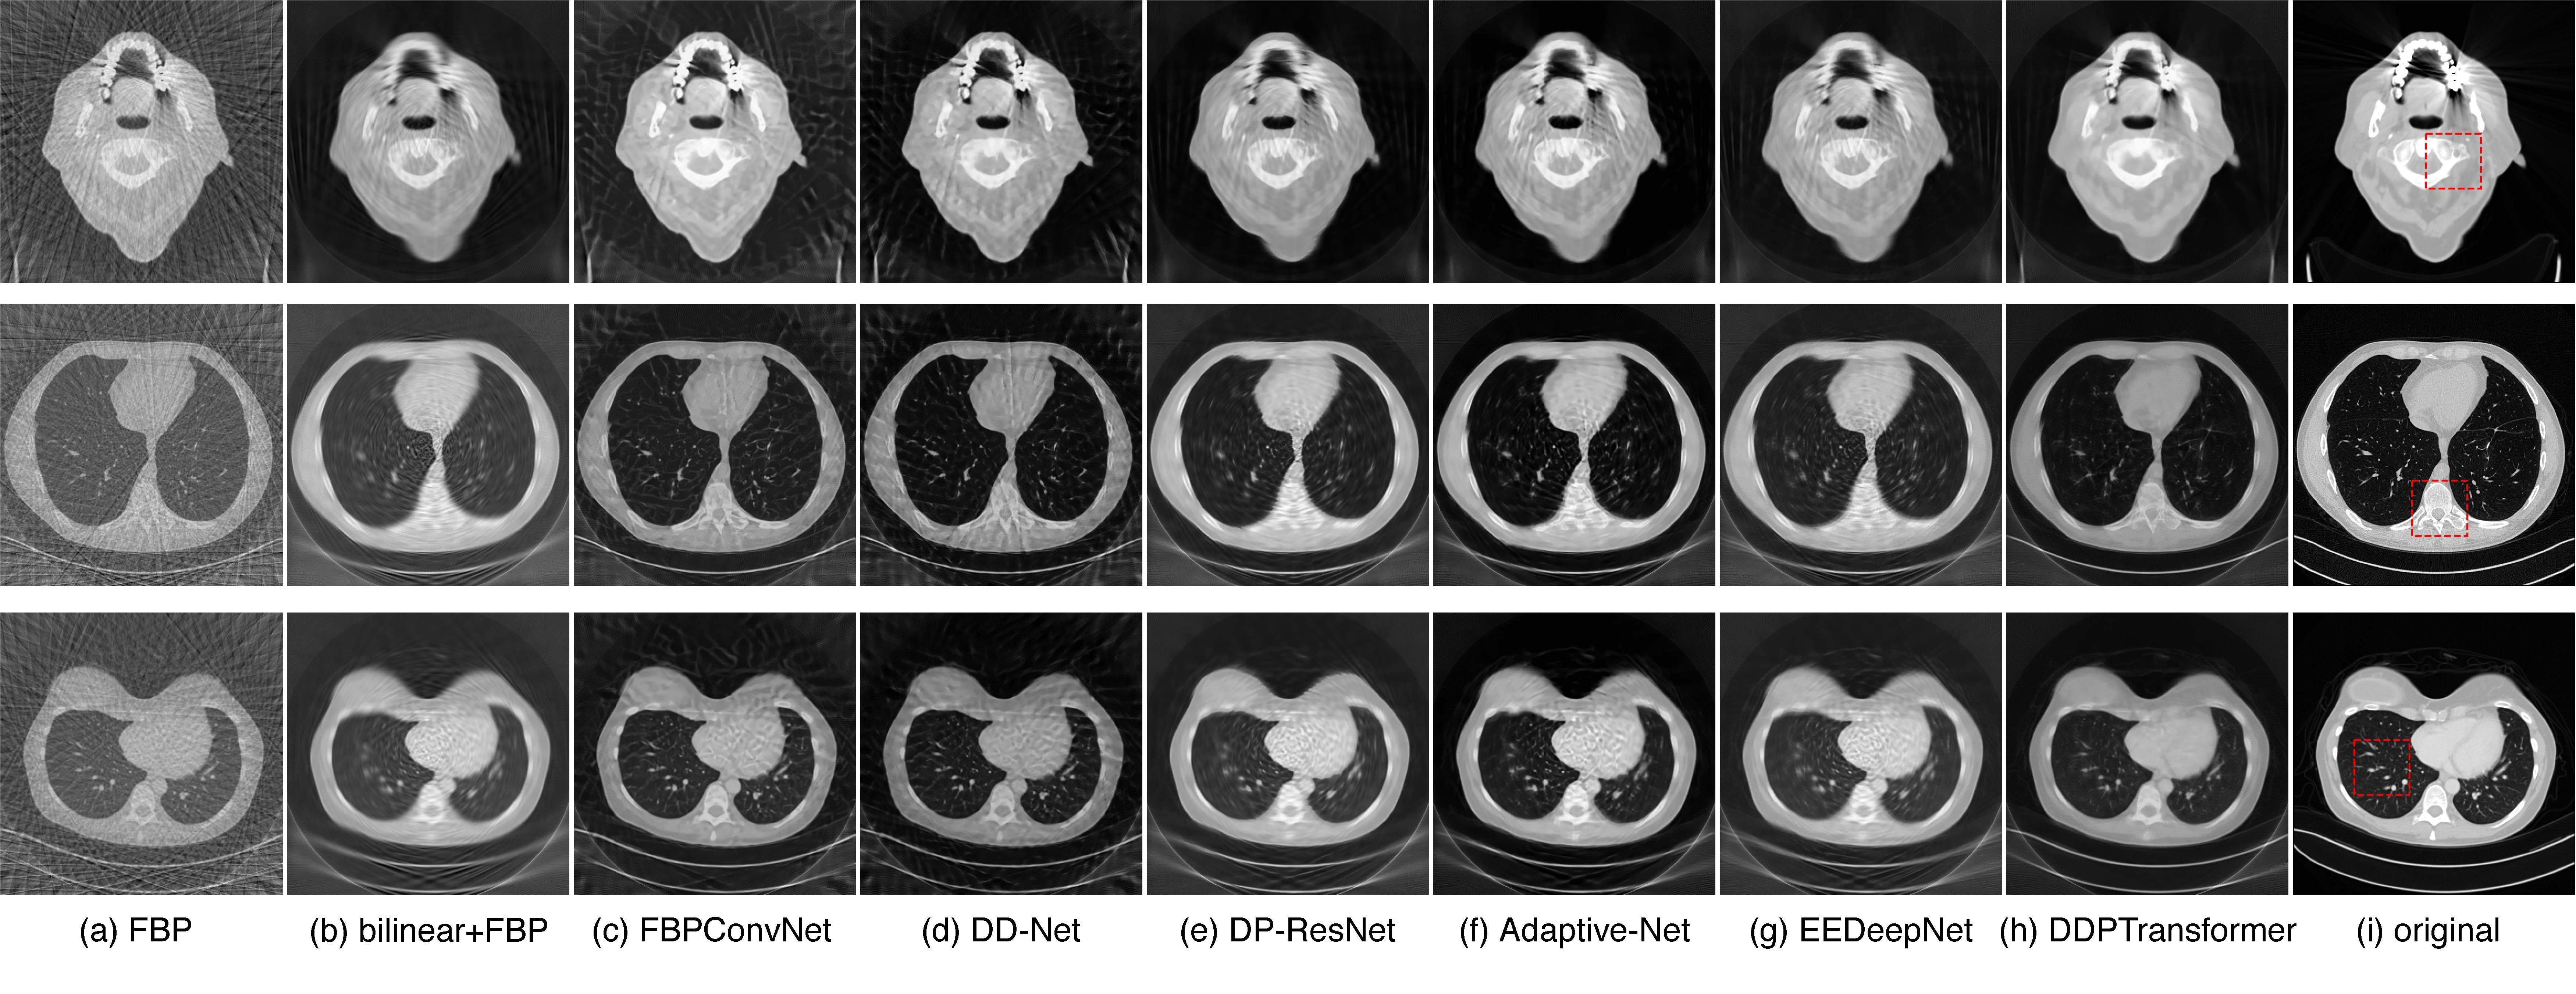
\includegraphics[height=6cm,width=18cm]{7.eps}
	\caption{64 views 不同器官的CT重建结果图。第一行是头部,第二行是胸部,第三行是腹部}
	\label{fig4}
\end{figure}
\begin{figure}
	\centering
	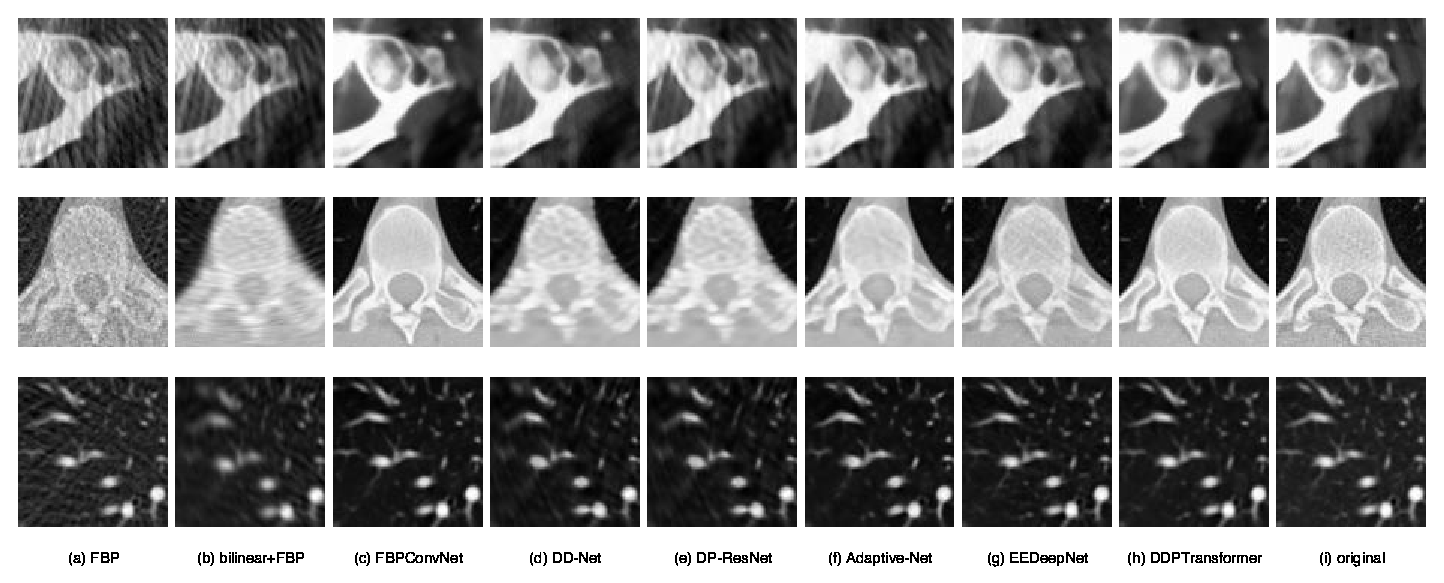
\includegraphics[height=6cm,width=18cm]{8.eps}
	\caption{128 views 不同器官的CT重建结果图。第一行是头部,第二行是胸部,第三行是腹部}
	\label{fig5}
\end{figure}
\begin{figure}
	\centering
	\includegraphics[height=8cm]{10.eps}
	\caption{图4和图5的评价指标,第一、二行分别为64、128views下不同的评价指标。n表示头部,c表示胸部,l表示腹部。}
	\label{fig6}
\end{figure}
\begin{figure}
	\centering
	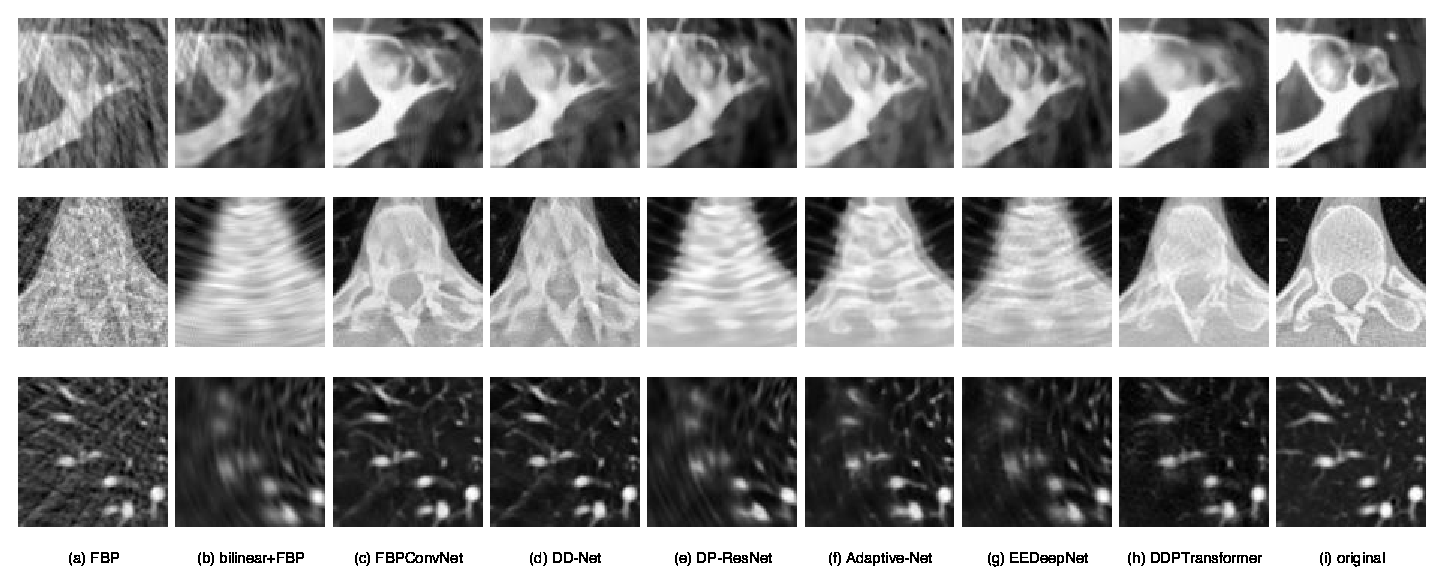
\includegraphics[height=7cm,width=18cm]{14.eps}
	\caption{图4(i)中红色框标记的缩放区域}
	\label{fig7}
\end{figure}
\begin{figure}
	\centering
	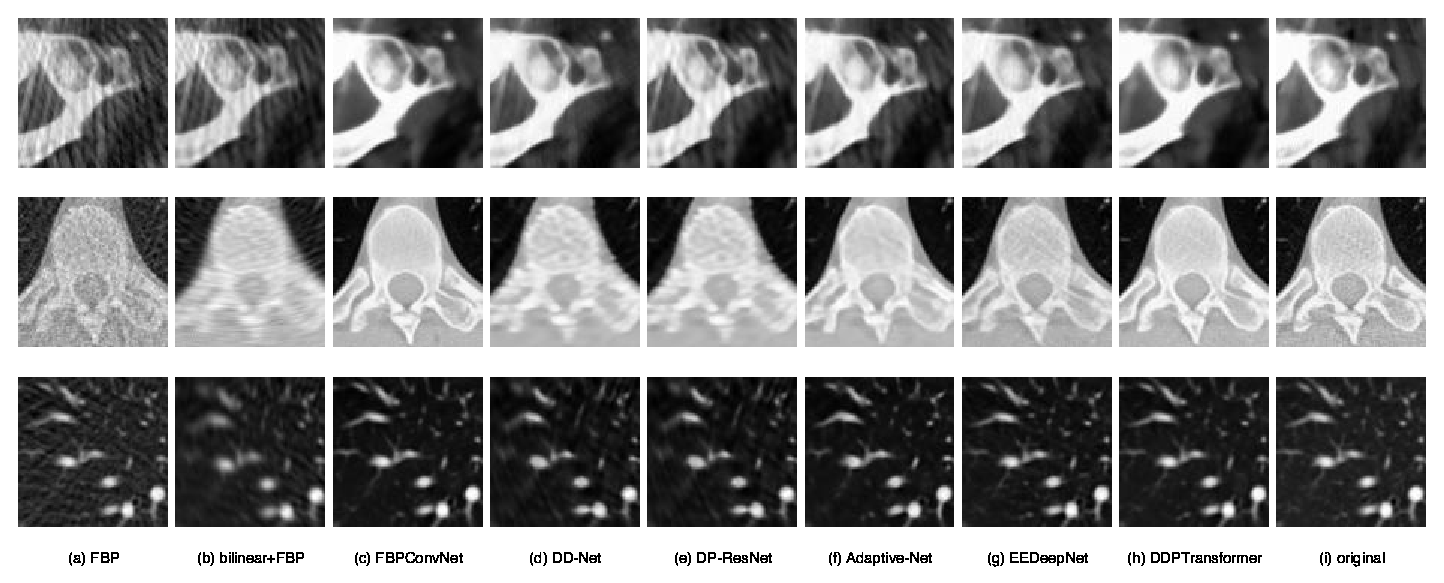
\includegraphics[height=7cm,width=18cm]{15.eps}
	\caption{图5(i)中红色框标记的缩放区域}
	\label{fig8}
\end{figure}

\subsection{Residual Plots}
为了进一步展示不同方法在定性分析上的结果,我们展示了与the original image相关的绝对差值图像(即残差图)和放大后ROI区域的残差图,并计算出了relative root mean square error (rRMSE).其公式如下:
\begin{equation}
\begin{aligned}
\mathrm{rRMSE(X,Y)} = \frac{\left\|X-Y\right\|_2}{\left\|Y\right\|_2} \times 100\%   
\end{aligned}
\end{equation}
where $X$ denotes the reconstructed image and $Y$ denotes the
corresponding reference image.rRMSE值越小表示残差部分在the reference image比重越少,即重建出的图像更接近于the reference image.图19\ref{fig19}显示了64 views下的重建结果,其中一、二、三行分别表示所选去的头部、胸部和腹部切片使用不同算法的重建结果,右上角红色矩形框表示放大后的ROI区域以及中下部分的蓝色框为相应的rRMSE值.很明显可以看出views过于稀疏,导致每个方法重建出的残差图都很明显.并且由FBPConvNet和DD-Net得到的残差图中存在大量的噪声.与DP-ResNet,Adaptive-Net和EEDeepNet相比,DDPTransformer得到的残差图轮廓更加不明显,说明在边缘细节的补充上有了很大的提升,并且消除了大多数噪声.进一步证明我们的模型在64 views上的定性分析结果最好.图20\ref{fig20}显示了128 views下的重建结果,同样一、二、三行分别表示头部、胸部和腹部使用不同算法的重建结果,右上角红色矩形框表示放大后的ROI区域以及中下部分的蓝色框为相应的rRMSE值.随着views的增加,每个模型得到的残差图效果更好。但DDPTransformer相比去其他方法产生了最小的差异,从而重建出的结果更加接近The Original Image.并且不管是64views还是128views下DDPTransformer在不同人体部分上都取得了最低的rRMSE值.
\begin{figure}
	\centering
	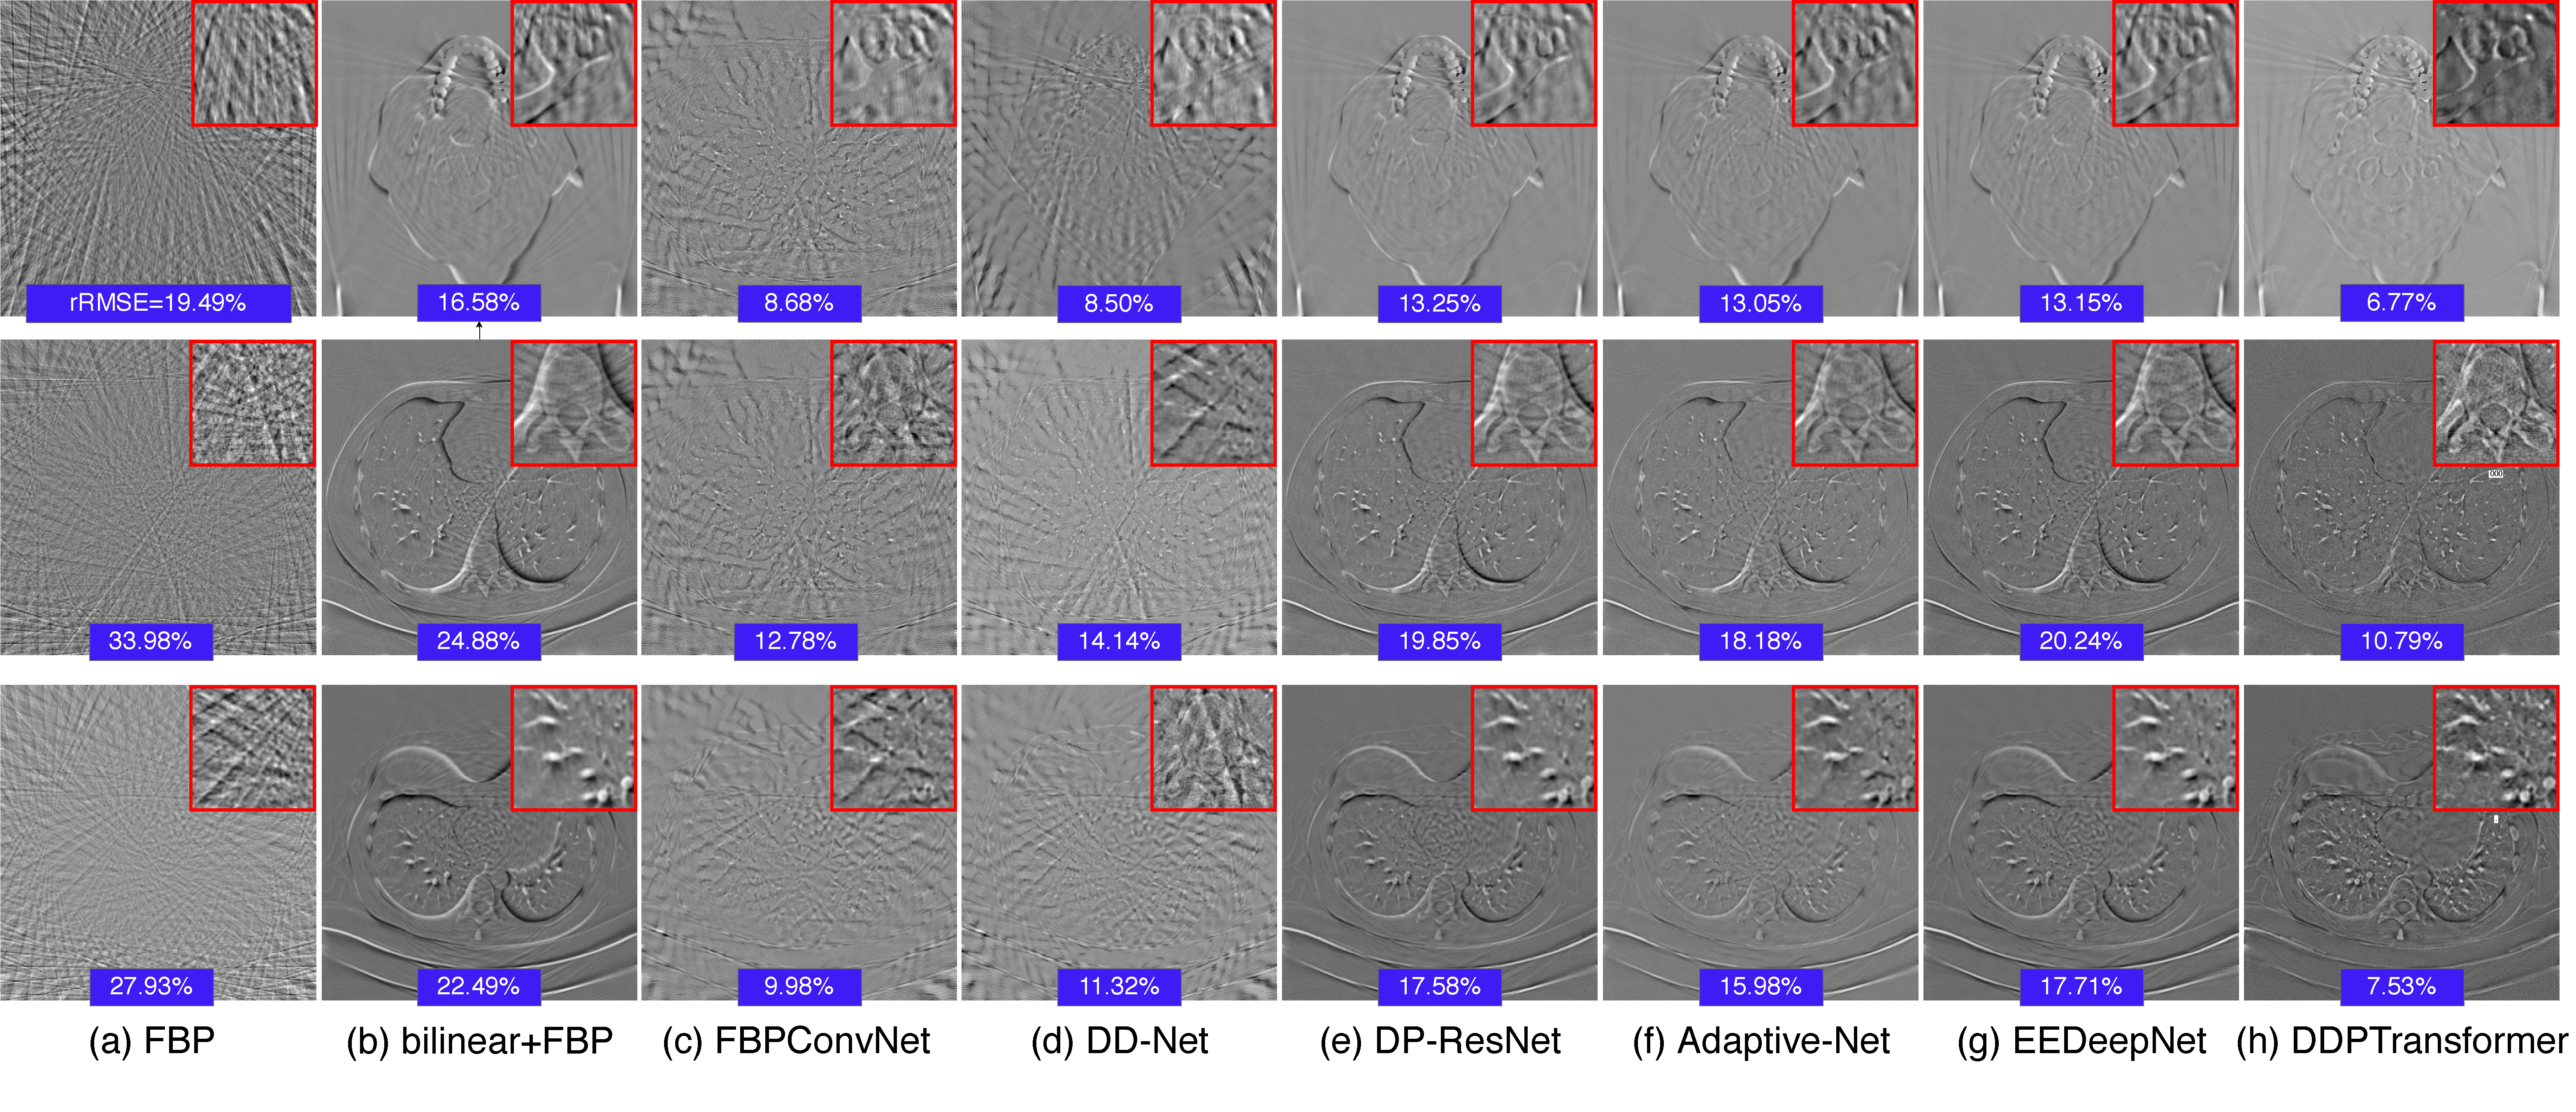
\includegraphics[height=7cm,width=18cm]{19.eps}
	\caption{absolute difference image relative to the original image under 64 views}
	\label{fig19}
\end{figure}
\begin{figure}
	\centering
	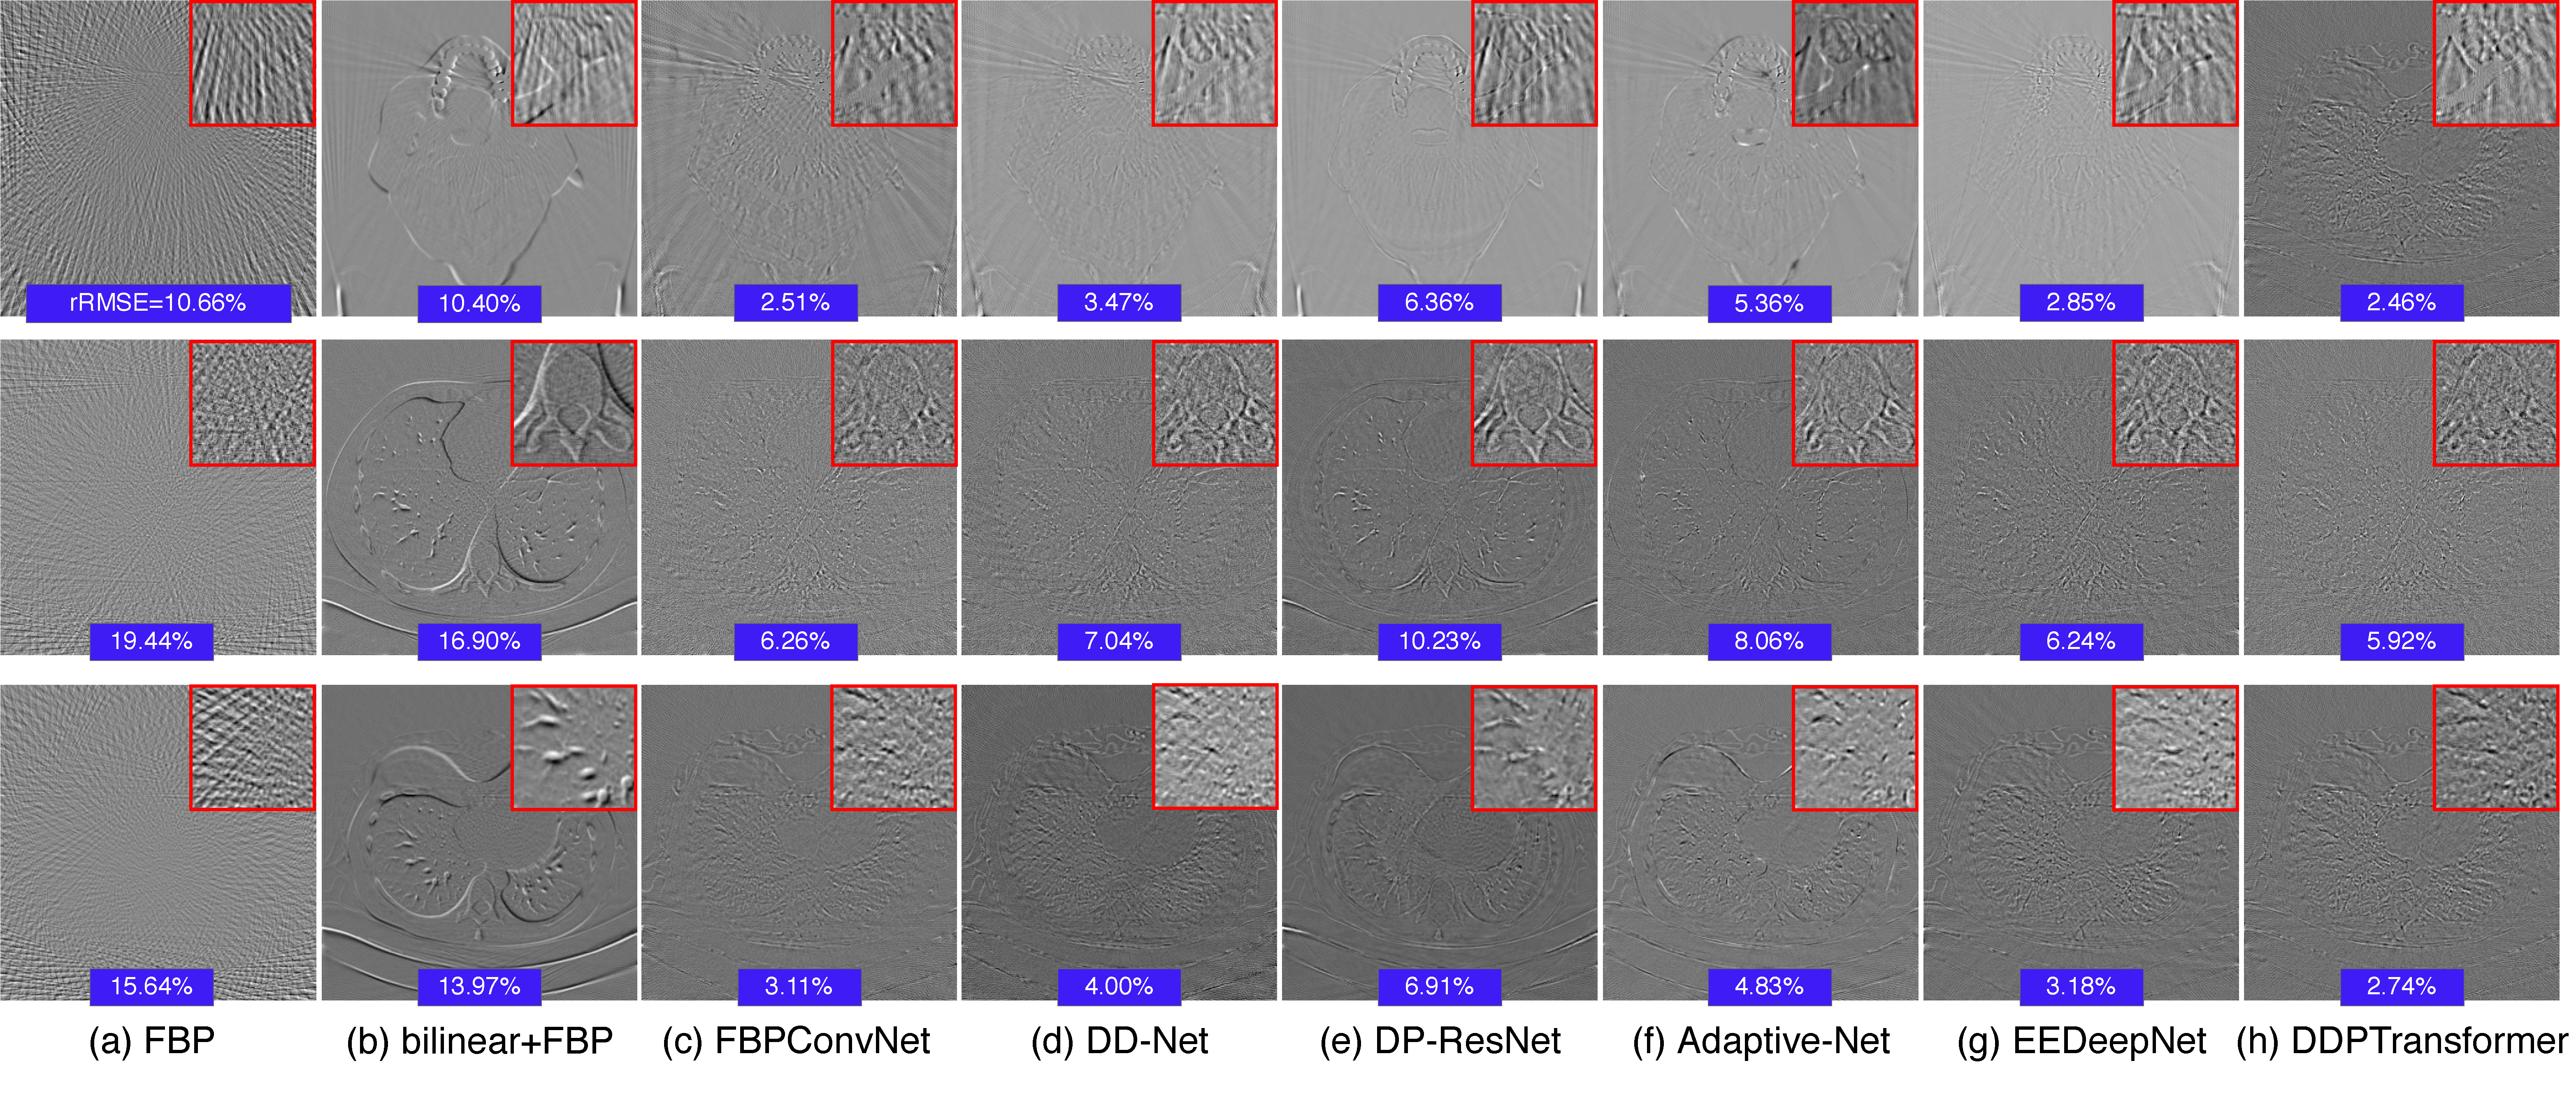
\includegraphics[height=7cm,width=18cm]{20.eps}
	\caption{absolute difference image relative to the original image under 128 views}
	\label{fig20}
\end{figure}

\subsection{Ablation Study}
在本节中,我们将评估DDPTransformer中不同组件的有效性。如验证Sinogram Domain SubNet(SD-Net)和Image Domain SubNet(ID-Net)的有效性;确定不同子网络中DDPTransformer block的个数$n$和$m$;以及验证并行Transformer和LCL模块的有效性。通过对一个参数进行改动,使其他参数保持不变,并对验证数据集的重构CT图像进行定量分析,确定各参数的最佳值。计算验证集中所有CT图像的PSNR、SSIM值和RMSE值。\par
\subsection{Effectiveness of Different SubNet}
我们分别对SD-Net和ID-Net的性能进行测试,它们的测试过程如图1\ref{fig1}(b)和(c)所示。表2\ref{tab2}列出了在不同采样下(views = 64 and 128)SD-Net和ID-Net重构出所有测试集的CT图像在性能评价结果上的均值和方差。可以看出ID-Net的重建效果要好于SD-Net,我们分析认为有两个主要因素导致ID-Net效果更好:一是相比于sinogram,CT图像本身具有更多的信息。二是为了更好的学习这些信息,ID-Net中DDPTransformer Block的个数要多于SD-Net。但可以看到由于无论哪一个子网络都无法达到DDPTransformer的性能评价指标。\par
\begin{table}[H]
	\centering
	\resizebox{\textwidth}{!}{ 
	\begin{tabular}{cccc|ccc}
		\hline
		method & PSNR & SSIM & RMSE*100 & PSNR & SSIM& RMSE*100 \\
		\hline  
		& \multicolumn{3}{c|}{64 views} & \multicolumn{3}{c}{128 views} \\
		\hline
		Sinogram Domain SubNet 
			& 28.9623$\pm$0.9575
			& 0.7297$\pm$0.0466
			& 0.1323$\pm$0.0273
			& 33.7763$\pm$1.5785
			& 0.8571$\pm$0.0383
			& 0.0453$\pm$0.0143 \\
		Image Domain SubNet 
			& 29.1686$\pm$0.3456
			& 0.7371$\pm$0.0172
			& 0.1235$\pm$0.0096
			& 33.7571$\pm$0.4986
			& 0.8597$\pm$0.0138
			& 0.0432$\pm$0.0049 \\
		DDPTransformer 
			& 29.6453$\pm$0.9910
			& 0.7590$\pm$0.0495
			& 0.1129$\pm$0.0236
			& 34.8335$\pm$1.8713
			& 0.8731$\pm$0.0385
			& 0.0362$\pm$0.0126 \\ 
			\hline
	\end{tabular}}
	\caption{子网络的性能评价结果(均值$\pm$方差)}
	\label{tab2}
\end{table}

\subsection{Number of DDPtransformer Blocks}
通过实验,我们将确定SD-Net中DDPTransformer Block的个数$n$,以及ID-Net中DDPTtransformer Block的个数$m$。我们根据所有测试集样本在性能评价结果上的均值进行判断,图10\ref{fig10}列出了根据$n$和$m$不同取值的折线图。其中第一行表示在SD-Net中的测试结果,我们设置$n$为从1到7,可以看出$n$从1到5时所有的评价指标效果都是越来越好,5之后效果趋于平稳,因此我们确定$n$的最佳取值为5。第二行表示在ID-Net中的测试结果,我们选择了$m$为从1到9进行实验,可以看出当$m$为7时,在64views上的SSIM和128view上的所有评价指标效果最好,以及在64views上的PSNR和RMSE效果也不错。并且考虑到块数过多可能会导致模型发生过拟合现象,所以综合考虑我们确定$m$的最佳取值为7。\par
\begin{figure}
	\centering
	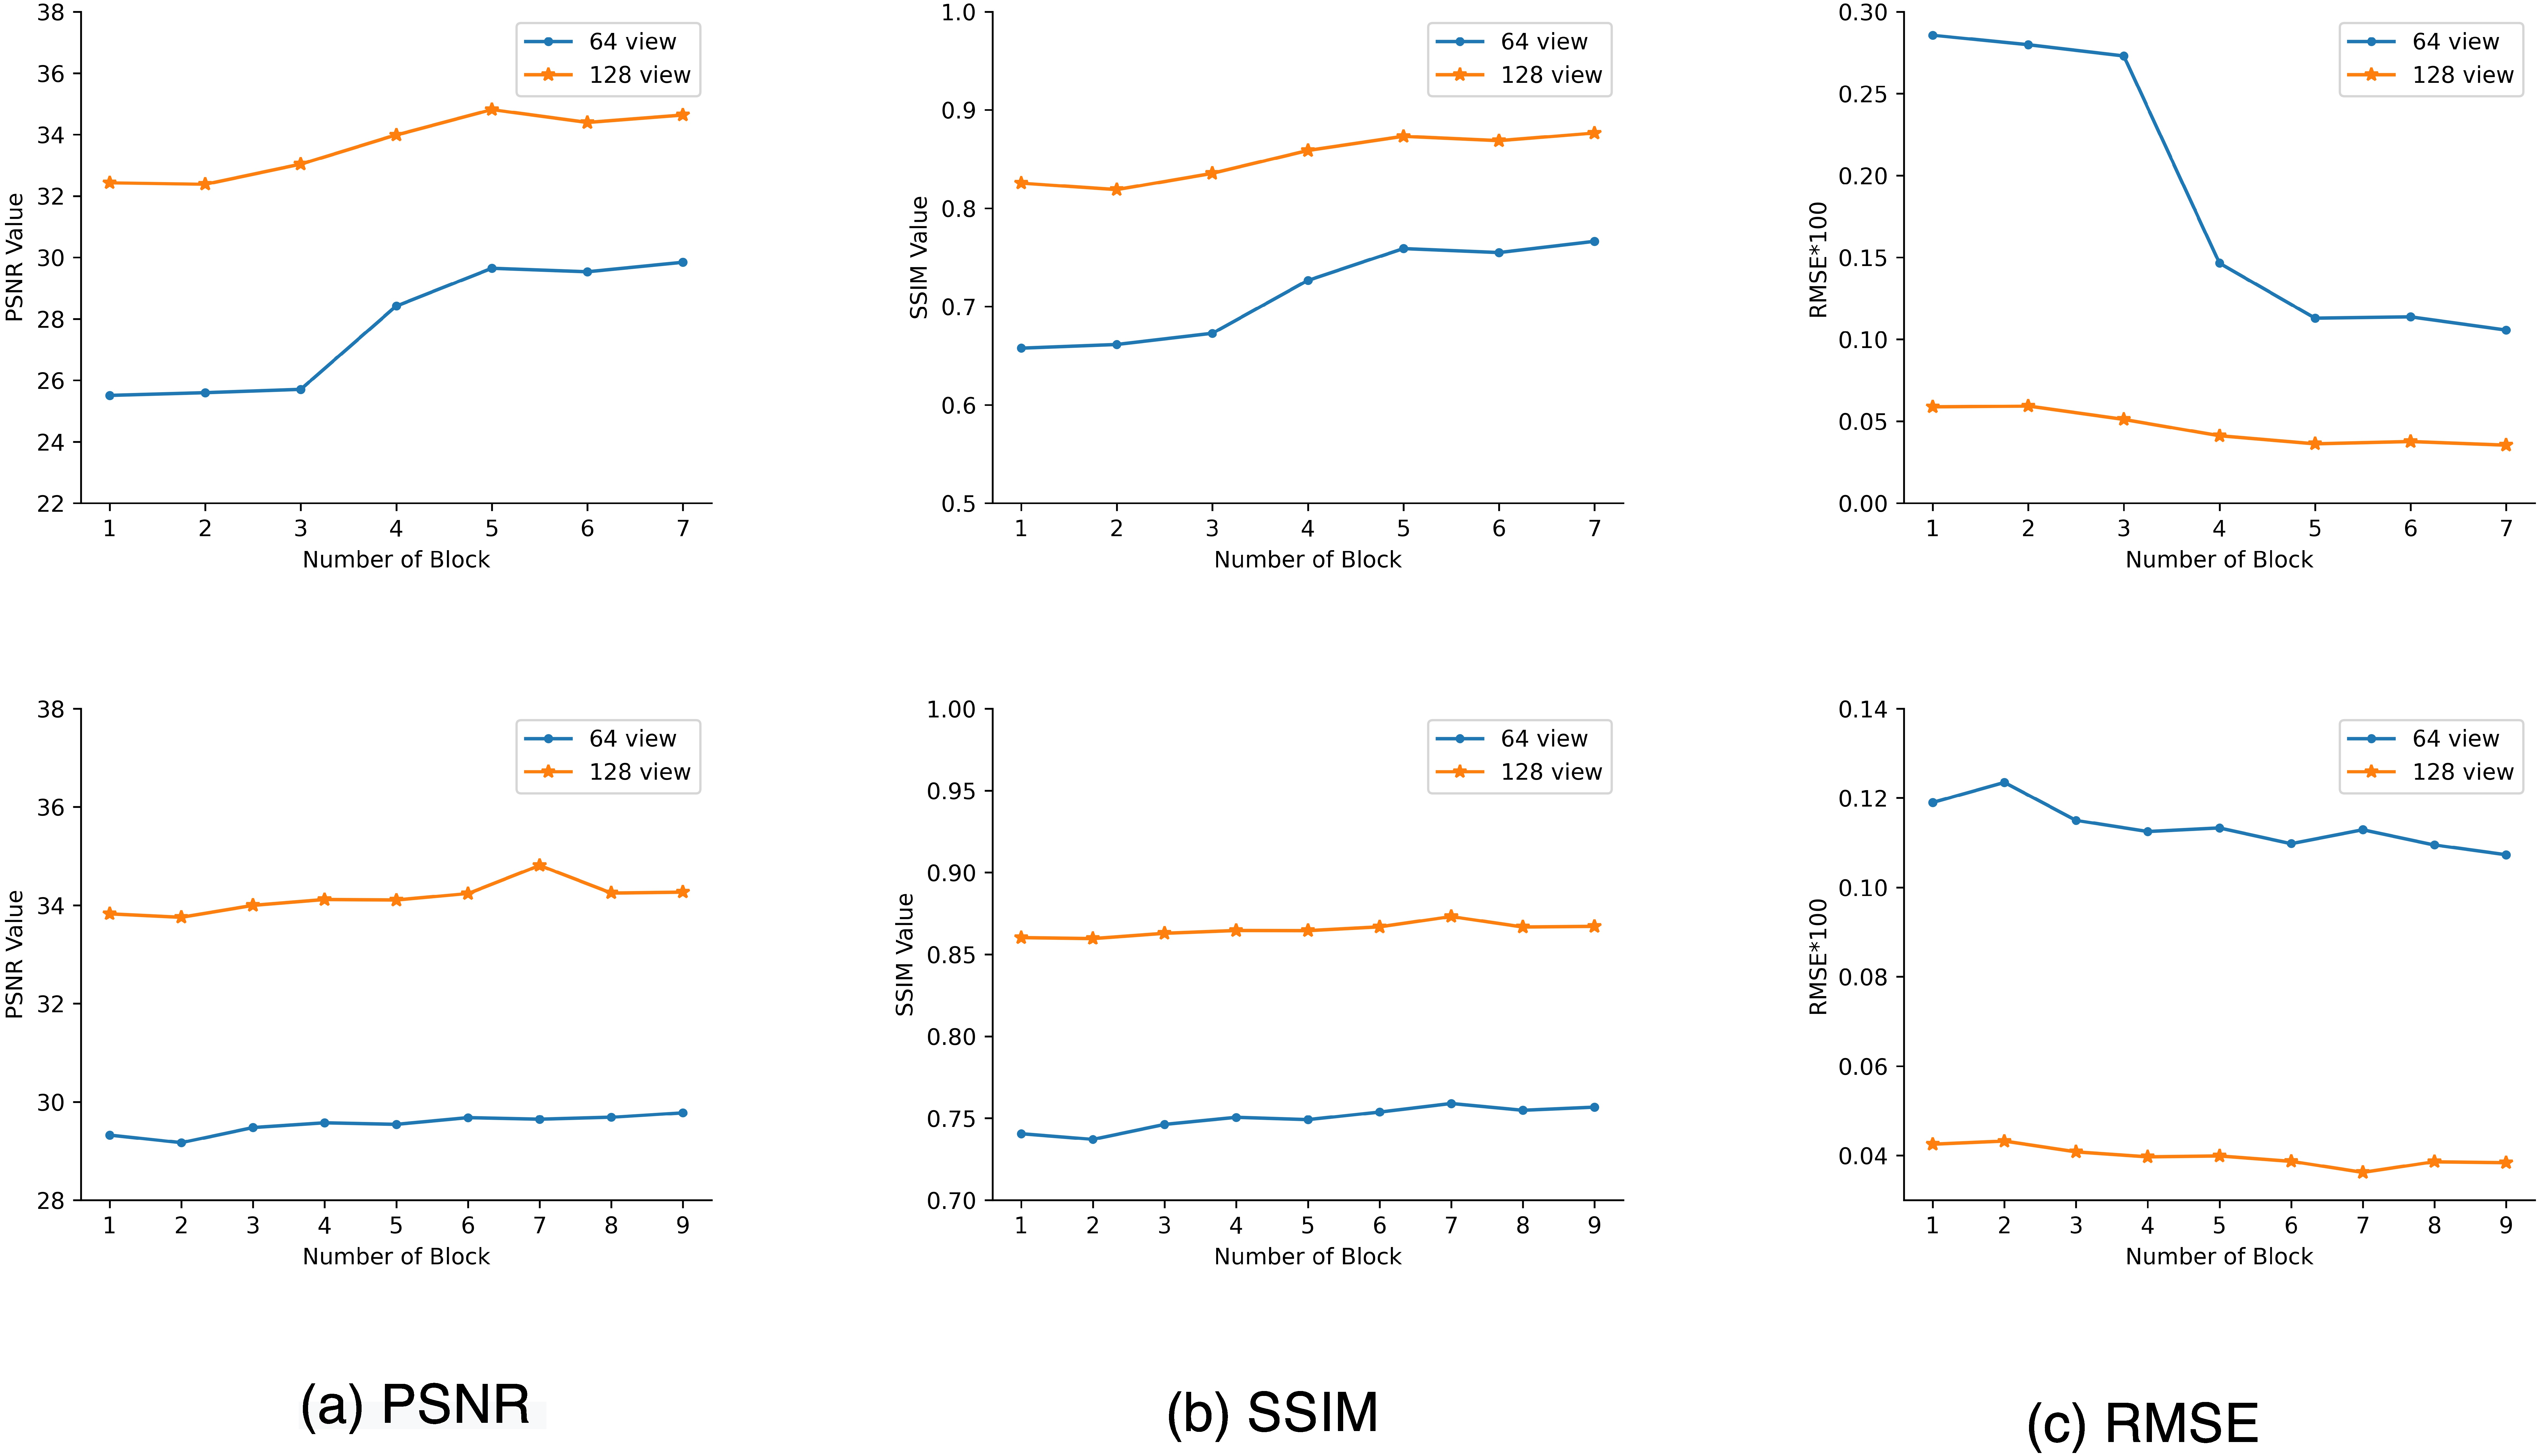
\includegraphics[height=8cm,width=15cm]{12.eps}
	\caption{Sinogram Domain SubNet(第一行)和Image Domain SubNet(第二行)中的block个数。}
	\label{fig10}
\end{figure}
\subsection{Effectiveness of Different Transformer}
本小节我们分别对DDPTransformer Block中的并行Transformer模块和LCL模块的有效性进行了实验验证.具体来说,验证的操作分别为:验证LCL模块对模型性能的影响时,我们将此模块改为MLP;验证并行Transformer对模型性能的影响时,我们将其改为串行Transformer;另外,我们还列出了单个Transformer+MLP以及串行Transformer+MLP作为对照组.我们根据所有测试集样本在性能评价结果上的均值和方差进行判断,结果如表3\ref{tab3}所示.将LCL模块改为MLP之后,我们可以看到不同的评价指标在不同的views上均有所下降,这说明LCL相比与MLP可以学习到图像更多的特征,从而可以重建出更好的结果;将并行Transformer改为串行Transformer之后,可以看到评价指标有更大幅度的下降,说明串行Transformer虽然解决了感受野有限的问题,但不同Patch的边缘信息并没有进行有效的互补,导致重建结果不如DDPTransformer.但不论LCL模块还是并行Transformer,与作为对照组的单个Transformer+MLP以及串行Transformer+MLP相比,性能均有不同程度的提升.实验结果证明了DDPTransformer Block中各个模块的有效性。\par
\begin{table}[H]
	\centering
	\resizebox{\textwidth}{!}{ 
		\begin{tabular}{cccc|ccc}
		\hline
		method & PSNR & SSIM & RMSE*100 & PSNR & SSIM& RMSE*100 \\  
		\hline
		& \multicolumn{3}{c|}{64 views} & \multicolumn{3}{c}{128 views} \\ \hline
		Single Transformer+MLP 
			& 27.4160$\pm$0.3170
			& 0.6693$\pm$0.0194 
			& 0.1848$\pm$0.0135
			& 30.9338$\pm$0.4125 
			& 0.7783$\pm$0.0164 
			& 0.0828$\pm$0.0077 \\
		Successive Transformers+MLP
			& 28.4761$\pm$1.0544
			& 0.7039$\pm$0.0537
			& 0.1488$\pm$0.0330 
			& 32.1355$\pm$1.4426
			& 0.8117$\pm$0.0447
			& 0.0656$\pm$0.0188 \\
		Successive Transformer+LCL
			& 27.8340$\pm$0.2849 
			& 0.7104$\pm$0.0170 
			& 0.1677$\pm$0.0107 
			& 32.7085$\pm$0.4841
			& 0.8350$\pm$0.0144
			& 0.0551$\pm$0.0060 \\
		DDPTransformer+MLP
			& 29.1885$\pm$1.0018 
			& 0.7155$\pm$0.0544 
			& 0.1257$\pm$0.0269
			& 32.5042$\pm$1.3632
			& 0.8110$\pm$0.0441
			& 0.0600$\pm$0.0165 \\
		DDPTransformer
			& \textcolor{red}{29.6453}$\pm$0.9910
			& \textcolor{red}{0.7590}$\pm$0.0495
			& \textcolor{red}{0.1129}$\pm$0.0236
			& \textcolor{red}{34.8335}$\pm$1.8713
			& \textcolor{red}{0.8731}$\pm$0.0385
			& \textcolor{red}{0.0362}$\pm$0.0126 \\ 
		\hline
	\end{tabular}}
	\caption{不同Transformer的性能结果 (均值$\pm$方差),最好的值用红色标出。}
	\label{tab3}
\end{table}

%\subsection{Running Time Comparisons}
%在NVIDIA RTX A5000 GPU上我们对运行时间进行测试。如表4\ref{tab4}所示,尽管与卷积相比Transformer在参数量、训练时间和难度上都有巨大的优势,但在单张切片上DDPTransformer的测试时间(即不计算梯度的反向传播算法)却与其他卷积网络相差不大。在几乎相同的运行时间中,DDPTransformer实现了卓越的性能。
%\begin{table}[H]
%	\centering
%	\begin{tabular}{cccccccc}
%		\hline
%		FBP & bilinear+FBP & FBPConvNet & DD-Net & DP-ResNet & Adaptive-Net & EEDeepNet & DDPTransformer\\ 
%		\hline
%		222 & 210 & 180 & 121 & 211 & 148 & 78 & 204 \\
%		\hline
%	\end{tabular}
%	\caption{不同方法的运行时间(单位:ms)}
%	\label{tab4}
%\end{table}
